We present the design and partial implementation%
\footnote{We had originally planned to realize this user interface as an extension of the existing frontend to the MathHub system.
However, this interface was based on Drupal, which led to a major system vulnerability when Drupal was repeatedly targeted by hackers.
Therefore, we are developing a new MathHub frontend from scratch, which has the advantage that the integration of Jupyter and MMT can be considered from the start.
It employs docker-based orchestration of services and a React.JS based frontend but is not publicly deployed just yet. We expect a fully-featured beta version until the OpenDreamKit Review end of November 2018. A development preview server is available at \url{http://new.mathhub.info}, but cannot be considered stable in any way.}
of a new user interface that combines the advantages of Jupyter Notebooks and MathHub documents.

\subsection{Architecture}

Our integrated VRE consists of four components: a Jupyter Notebook server\footnote{\url{http://jupyter.mathhub.info}}, a MathHub Git repository hosting server\footnote{\url{http://gl.mathhub.info}}, an MMT instance\footnote{\url{http://mmt.mathhub.info}}, and our new MathHub frontend\footnote{To be deployed at \url{http://mathhub.info}; development preview at \url{http://new.mathhub.info}} that serves as the main entry point for users and delegates some subtasks to the former.
The Jupyter server is an out of the box installation of Jupyter except for additionally supporting our new MMT kernel.
Jupyter Notebooks are stored (and versioned) as regular files in MathHub.

The MathHub frontend provides special interaction functionality for individual document types.
This allows making Jupyter Notebooks a new document type; see Figure~\ref{fig:mathhub-NB} for an example.
When displaying a known document type, the frontend shows multiple tabs.
For notebooks, these are the following:
\begin{compactenum}[\em i\rm)]
\item \textsf{view} gives a preview of the notebook, essentially the computation cells without output, pre-rendered for static serving without involving Jupyter at all.%
\ednote{MK: we should implement this; I am not sure what the best way is for this. I guess a build target based on \texttt{https://github.com/jendas1/jupyter-notebook-quick-look}.}
\item \textsf{run/edit} opens the respective notebook on the Jupyter server for execution and editing.
Any changes to the notebook can be committed back to the Git repository. 
\item \textsf{metadata} (this is the tab open in Figure~\ref{fig:mathhub-NB}), shows the metadata provided by the Jupyter kernel and the repository. 
\item \textsf{source} provides access to the document source; here simply a link to the notebook file in the Git repository.
\item \textsf{statistics} shows statistical information about the notebook, its corresponding MMT document, and its connections with other MMT documents in the background knowledge base.
\item \textsf{graph} links to graph-based visualizations of the document including the theory graph, declaration graph, and dependency graph, using our TGView system, a canvas-based in-browser visualizer for knowledge graph information~\cite{RupKohMue:fitgv17}.
\end{compactenum}
This integration combines the interactive features of the Jupyter server with the knowledge management facilities on MathHub. In the future, we plan to integrate the notebook diff/patch \textsf{nbdime} developed in OpenDreamKit to extend the knowledge management facilities. 

\begin{figure}[ht]\centering
  \fbox{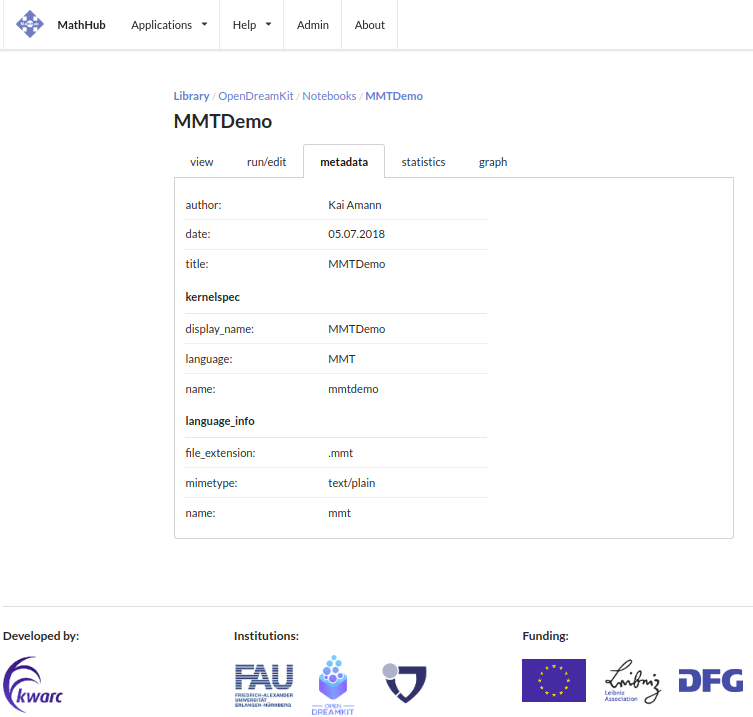
\includegraphics[width=13cm]{../D4.11/NB-Mathhub}}
  \caption{A Jupyter Notebook in MathHub.info (Metadata)}\label{fig:mathhub-NB}
\end{figure}

%A Jupyter Notebook additionally has a special button appears that allows users to open the notebook in the associated Jupyter server. Currently these notebooks do not use the MMT process running on MathHub.info, due to the architecture of the MMT Kernel. Therefore they currently do not have access to the MathHub universe. \ednote{KA: if the Kernel server would run on the same VM as the MathHub MMT we could give the kernel access to it}
%\ednote{@Kai, @Tom: check this, do the implementation}

\ednote{@KA: write the example from Fig.~\ref{fig:test_theory} as a Jupyter notebook, store the file somewhere on gl.mathhub.info and give a link to the Fig.~\ref{fig:mathhub-NB} view of that notebook}

\subsection{Document/Notebook Integration}

To achieve full document/notebook integration, as envisioned in D4.2~\cite{ODK-D4.2}, we have developed a tool that generates ephemeral Jupyter Notebooks dynamically and embeds them into HTML presentation of MathHub documents.
Here we can feed the document context information into the interior notebook as described in~\cite{ODK-D4.9} (this part of the integration can be re-used directly).

\begin{figure}[ht]\centering
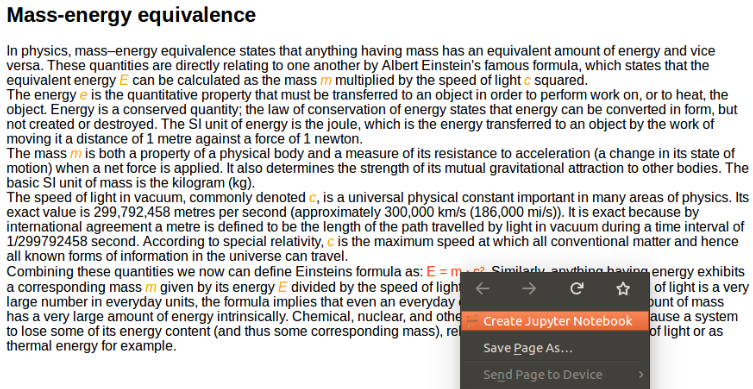
\includegraphics[width=15cm]{../D4.11/conversionHTML}
\caption{HTML document and the context menu for converting}
\label{fig:conversionHTML}
\end{figure}

As a running example, we revisit the active computation example from the previous section.
Figure~\ref{fig:conversionHTML} shows an example of a scientific HTML document that contains the equation $E=mc^2$.
The user can use the context menu to trigger the notebook generation on this formula.
The context menu is generated using Javascript that picks up on annotations of formulas with specific CSS classes.
Currently the author has to manually annotate the formulas, but we are working on a mechanism to automatically create it from the document context.

Figure~\ref{fig:conversionNotebook} shows the notebook created by our tool.
If desired, the notebooks can be easily uploaded to the Jupyter server, stored persistently in the repository server, or evaluated in a locally deployed version of the system per drag-and-drop.

Note that the generated notebook starts with several \texttt{include} declarations that import the context of the formula.
These are generated by MathHub to obtain a minimal standalone MMT theory in which the respective formula is well-formed. 

%The two predominant cell types in Jupyter notebooks are \texttt{code} and \texttt{markdown} cells. 
%Code Cells contain user input, like described in section \ref{sec:kernel:syntax}.
%The HTML elements that contain the input for these code cells are usually not visible, since they do not fit into the context of a scientific document and may not be understood by reviewers that are not familiar with MMT syntax. 
%The other cell type: markdown cells, can contain any type of plain text and support GitHub flavoured markdown. 
%Therefore markdown cells are used for providing notebooks with additional selectable information from the original HTML document.
\ednote{MK@KA/FR: For the evaluation (and Kai's thesis) we should make an sTeX document that contains $E=mc^2$ (e.g. by copying parts of \texttt{https://en.wikipedia.org/wiki/Mass-energy\_equivalence}) and really implement the in-document computation example. This would make a wonderful demo in Brussels.}

\begin{figure}[ht]\centering
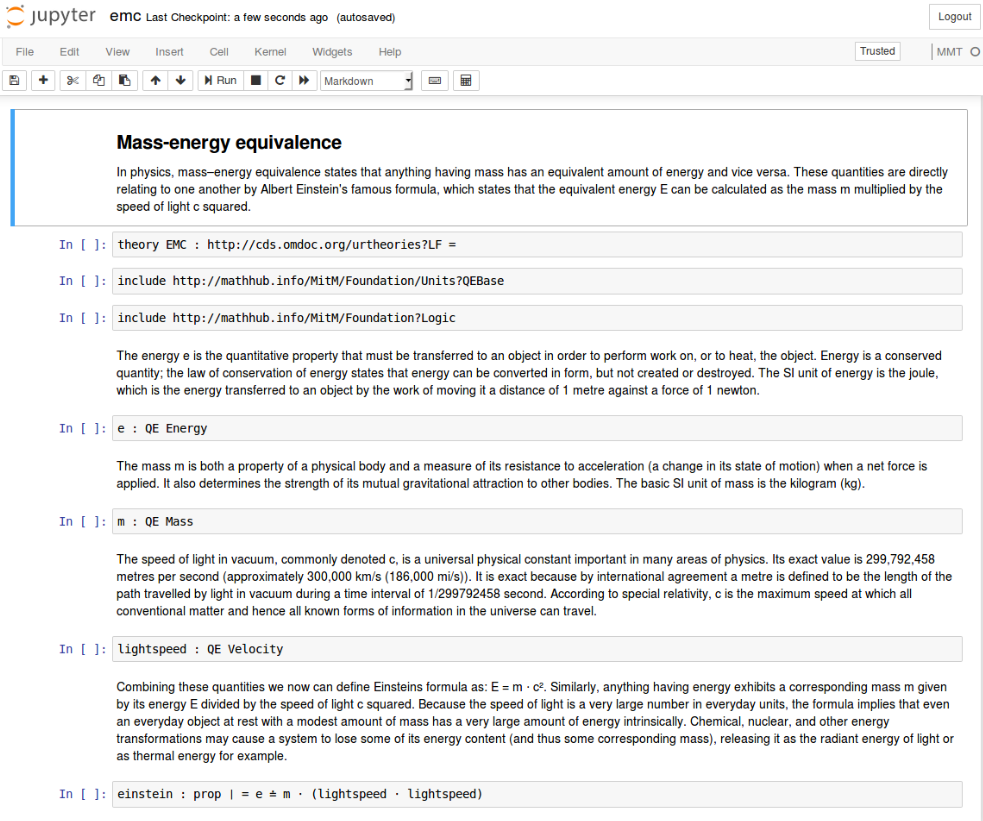
\includegraphics[width=15cm]{../D4.11/conversionNotebook}
\caption{The resulting Jupyter notebook}
\label{fig:conversionNotebook}
\end{figure}


%%% Local Variables:
%%% mode: latex
%%% mode: visual-line
%%% fill-column: 5000
%%% TeX-master: "paper"
%%% End:

%  LocalWords:  Jupyter ednote compactenum textsf texttt visualizations RupKohMue:fitgv17 nbdime centering fbox includegraphics NB-Mathhub
